\chapter{Procedure Design Methodology}
\section{Input Stage}
The input stage of the amp testing procedure was the first to be targeted. Directing input to the amp card should be a simple task for the user. Since all four channels are used in parallel on the system, they can be connected to a unified signal source and displayed together on the oscilloscope for data collection. Using a mix of hardware and software support I developed an input procedure for the new test.
\subsection{Function Generation}
To implement a Python layer for the function generator I opted to use a FeelTech FY6900 Arbitrary Waveform Generator.
\begin{figure}[!htb]
	\centering
	\includegraphics*[]{awg}
	\caption{FeelTech FY6900}
\end{figure}
This was a relatively cheap function generator that fulfilled the tasks we needed to accomplish. With up to 60MHz sine wave output, this device was more than enough to test the capabilities of the amplifiers. The DAC input the amps were designed to process were at frequencies far below this. For the first versions of the test I opted to use the original function generator settings until more could be determined about the input parameters. The code was simple and based on the previously listed libraries \& protocols:
\begin{lstlisting}
	awg.set_on_off(1, 0)
	awg.set_on_off(2, 0)

	awg.set_waveform(1, 1)
	awg.set_frequency(1, 1000000)
	awg.set_amplitude(1, x[i])
	awg.set_offset(1, 0.318)
	awg.set_phase(1, 0)

	# Turn channel 1 on
	awg.set_on_off(1, 1)
\end{lstlisting}
For the automated test to save time, it was set to loop four times to collect plot data from the oscilloscope for all four amplifier output channels. In order for this automatic switching to work, hardware had to be designed to accept the signal and distribute it accordingly.
\subsection{Bottom (Input) PCB}
Major flaws in the original test setup included the lack of any shielded cable to transfer the input signal and the tester having to manually clip the input to each amp channel. Although we were not necessarily testing for strict signal integrity, it is better practice to use standard connectors for input rather than probe clips. Since the FeelTech generator used a BNC connector it was easiest to match this on the input card. BNC connectors are shielded coaxial connectors capable of reliably passing signals under 4GHz and less than 500V \cite{bncbook}. \par
Separating the amplifier's input lines was a useless step that only served to complicate the process. To solve this I had to examine the amp's PCB layout to find the relevant pins. The DAC inputs were differential pairs identified within the layout below:
\begin{figure}[!htb]
	\centering
	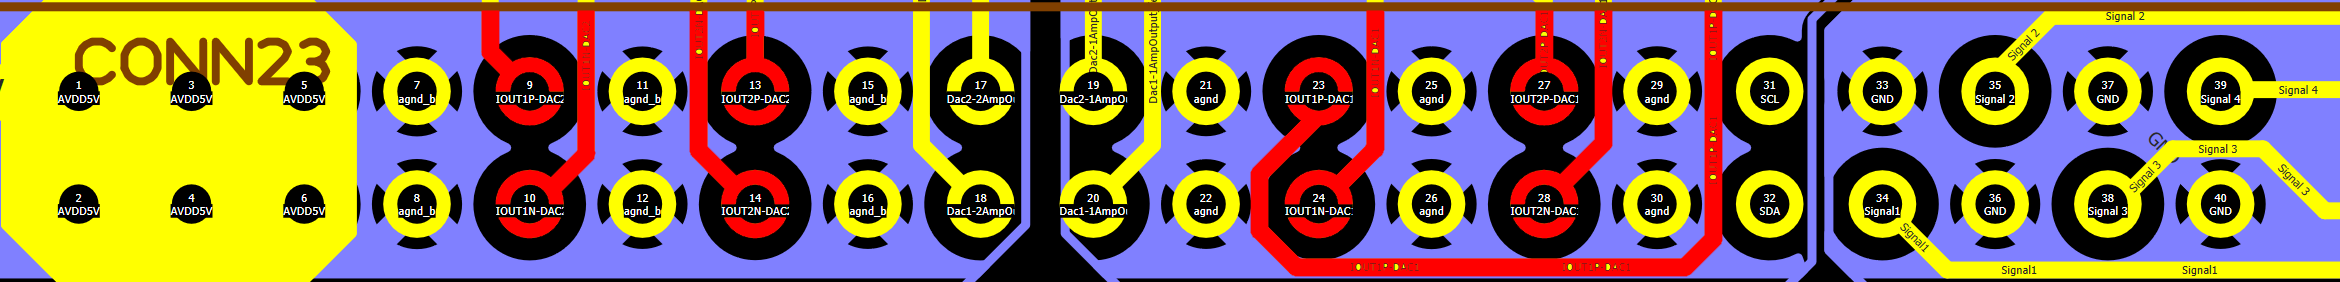
\includegraphics[width=\textwidth]{amp_input_pins}
	\caption{Differential input pins on the Amp PCB}
\end{figure}
The input side of the board was fairly simple to draw and lay out. One of the amp's purposes was to turn the DAC's differential output into a single-ended output. To accomplish this, the amp card terminated the N-terminals of all incoming DAC signals through a 49 ohm resistor.
\begin{figure}[!htb]
	\centering
	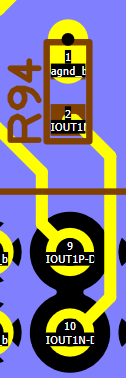
\includegraphics{amp_n_p}
	\caption{Terminating resistor for the N-terminal of the DAC output.}
\end{figure}
Grounding the differential input was an acceptable decision for the test setup. Only the P-lines of the signal would be processed by the circuit at all, so they were routed together and joined to a single BNC input in the test board.
The layout followed shortly and included a ground plane to maximize signal integrity. With such a limited number of relevant pins on the input side of the amp card, designing the test board was not an issue. \par
\subsection{Input Conclusion}
This section of the test setup resulted in a far simpler procedure. Having to only connect one output through a stable connection and clearly labeled board eliminated all possible confusion for testers.
\begin{figure}[!htb]
	\centering
	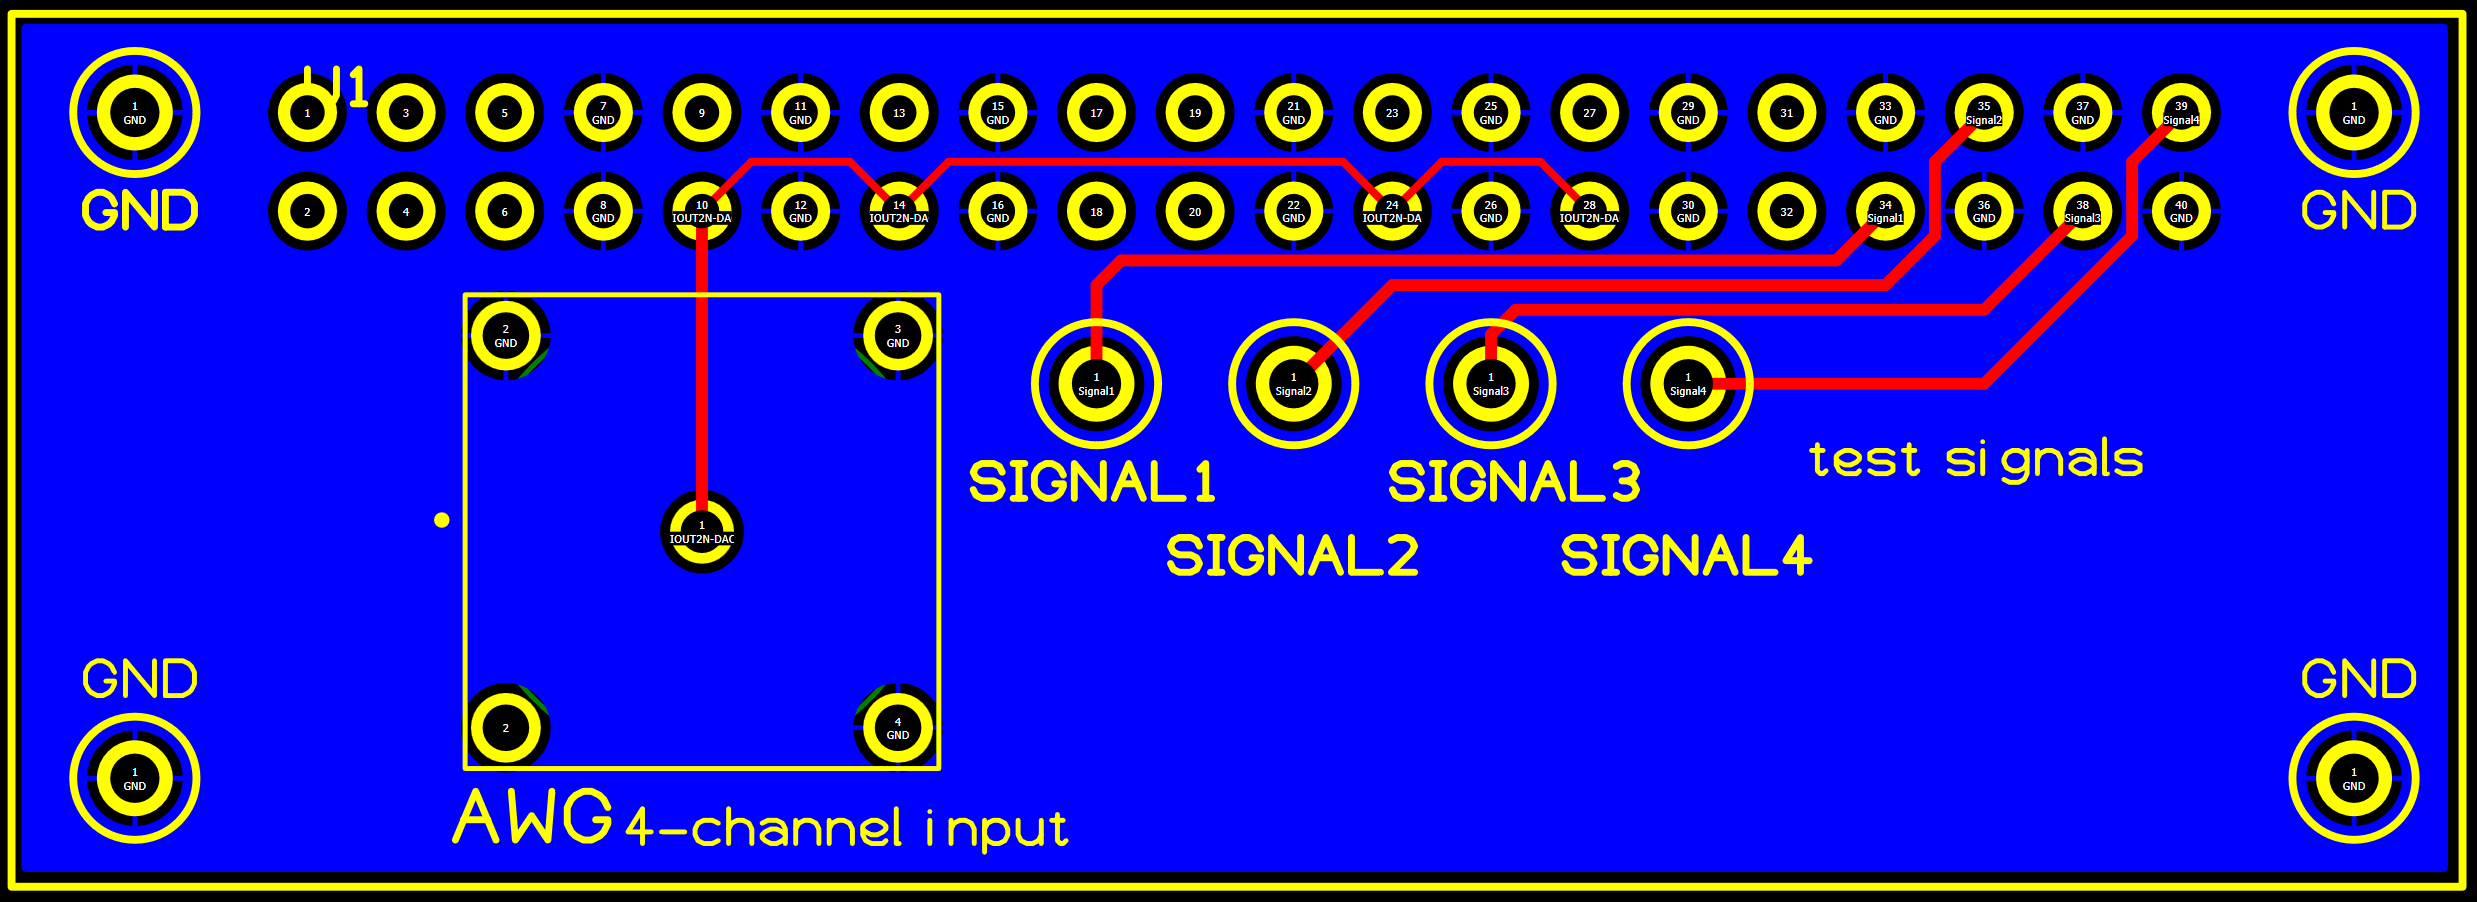
\includegraphics[width=\textwidth]{amp_bottom_layout}
	\caption{Input Test board layout}
\end{figure}
\begin{figure}[!htb]
	\centering
	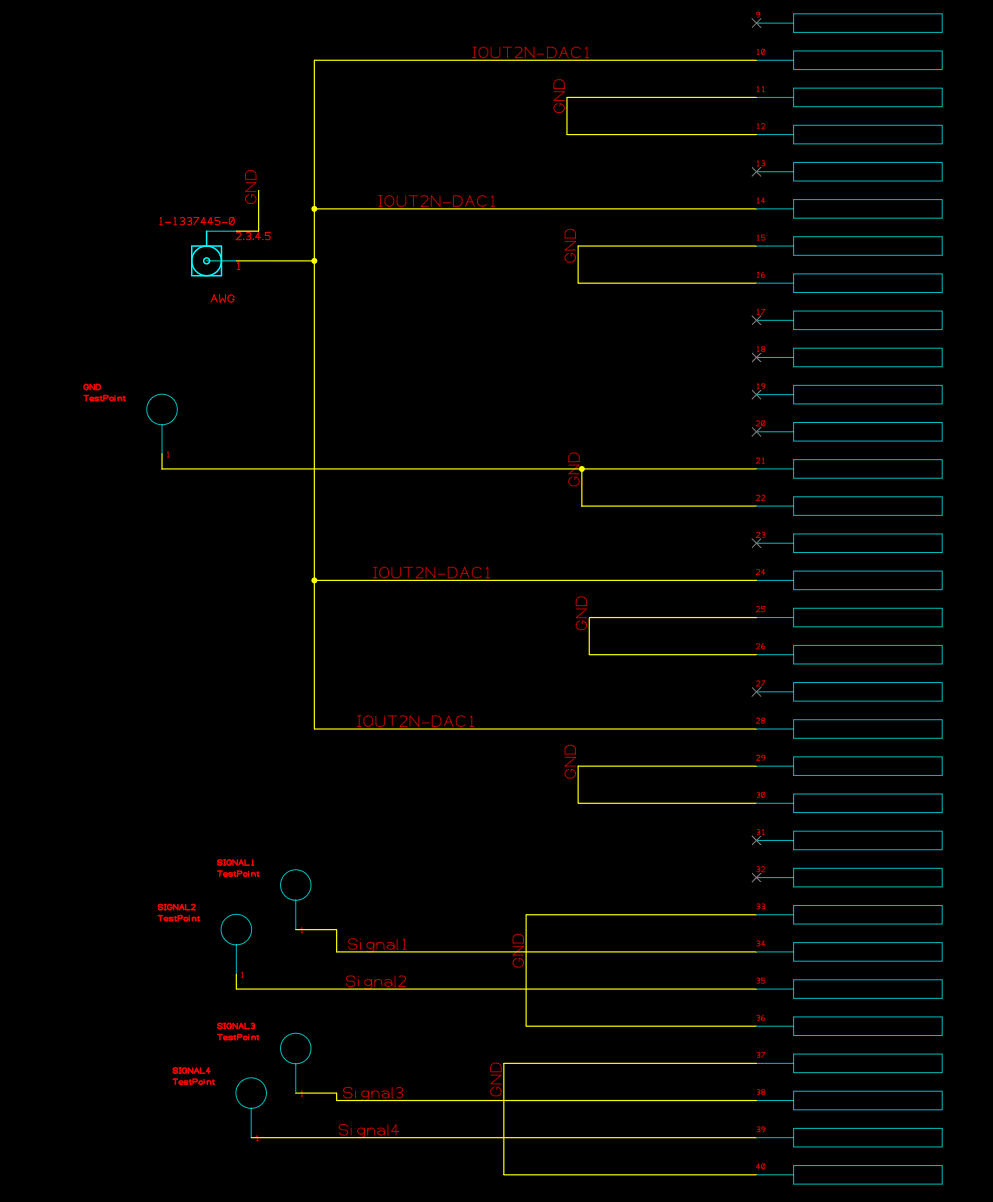
\includegraphics[width=\textwidth]{amp_bottom_schematic}
	\caption{Input Test board schematic for joining P-inputs and grounding N-inputs}
\end{figure}
\begin{figure}
	\centering
	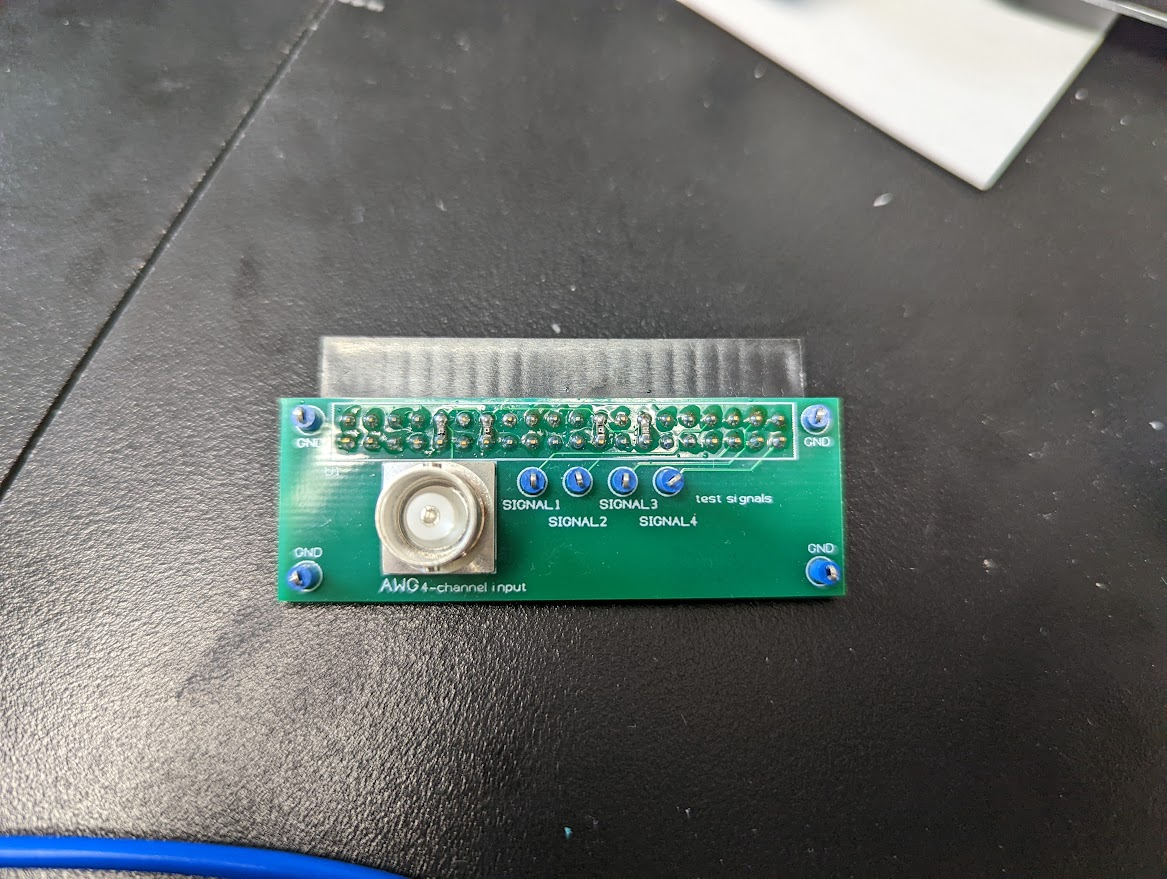
\includegraphics[width=\textwidth]{amp_bottom_board}
	\caption{Final fabricated bottom test board}
\end{figure}
\begin{figure}
	\centering
	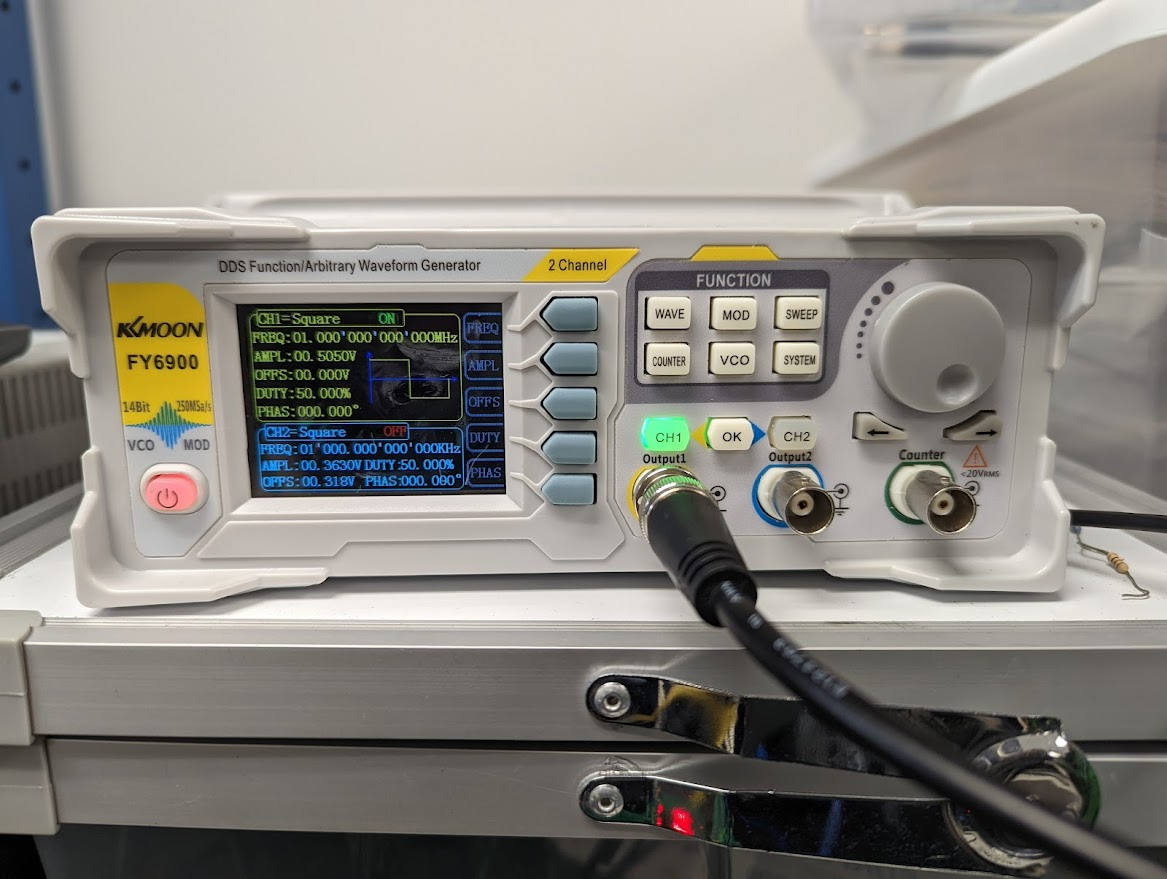
\includegraphics[width=0.7\textwidth]{function_gen_programmed}
	\caption{Oscilloscope with desired settings programmed}
\end{figure}

\section{Output Stage}
The output of the amp card required the testers to be able to view all output channels at once as well as collect and plot the oscilloscope's data. This once again required a mix of software and hardware tools to accomplish.
\subsection{Top (Output) PCB}
Before any data could be routed to the oscilloscope we needed to develop a control system for the top connector of the amp card. This connector housed a number of vital pins including power rail input and amplifier output. In the system, this connector would be attached to the interface board and transport signals through the ribbon cables. To appropriately test the functionality of all amp cards, users had to be able to fulfill a number of requirements:
\begin{itemize}
	\item Ensure power was being properly delivered to both amplifiers
	\item Have the ability to independently toggle power to each amplifier unit
	\item Route output through shielded cable to oscilloscope
\end{itemize}
Each section of the PCB was therefore designed to address these issues. To indicate valid power delivery a simple LED indicator system was sufficient. Each amplifier had its own pin for power delivery and as such could be routed independently. A switch with three positions was used to control power delivery. When in neutral, power would be routed to both amplifiers A and B. When flipped left or right, the switch would direct power into only amplifier A or B respectively. The LED indicators were placed into voltage dividers. If enough voltage was being delivered on that line, the divider would pass voltage to light up the LED. \par
When moving on to the layout the main concern was for space and signal integrity. By keeping the board as symmetrical as possible and including another ground plane, the design was ensured to be safe from interference. The four output channels were available as BNC headers as well and could be directly connected to a 4-channel oscilloscope. The switch and LED components provided the most challenges in layout as they required quite a few traces. The final layout was compact and clearly labeled to show testers what they needed to use. Power delivery was accomplished through probe clips to the power supply. The power supply is never changed or adjusted during the whole process, so the clips were not any issue when detatching and reattaching cards from the testing boards.
\begin{figure}[!htb]
	\centering
	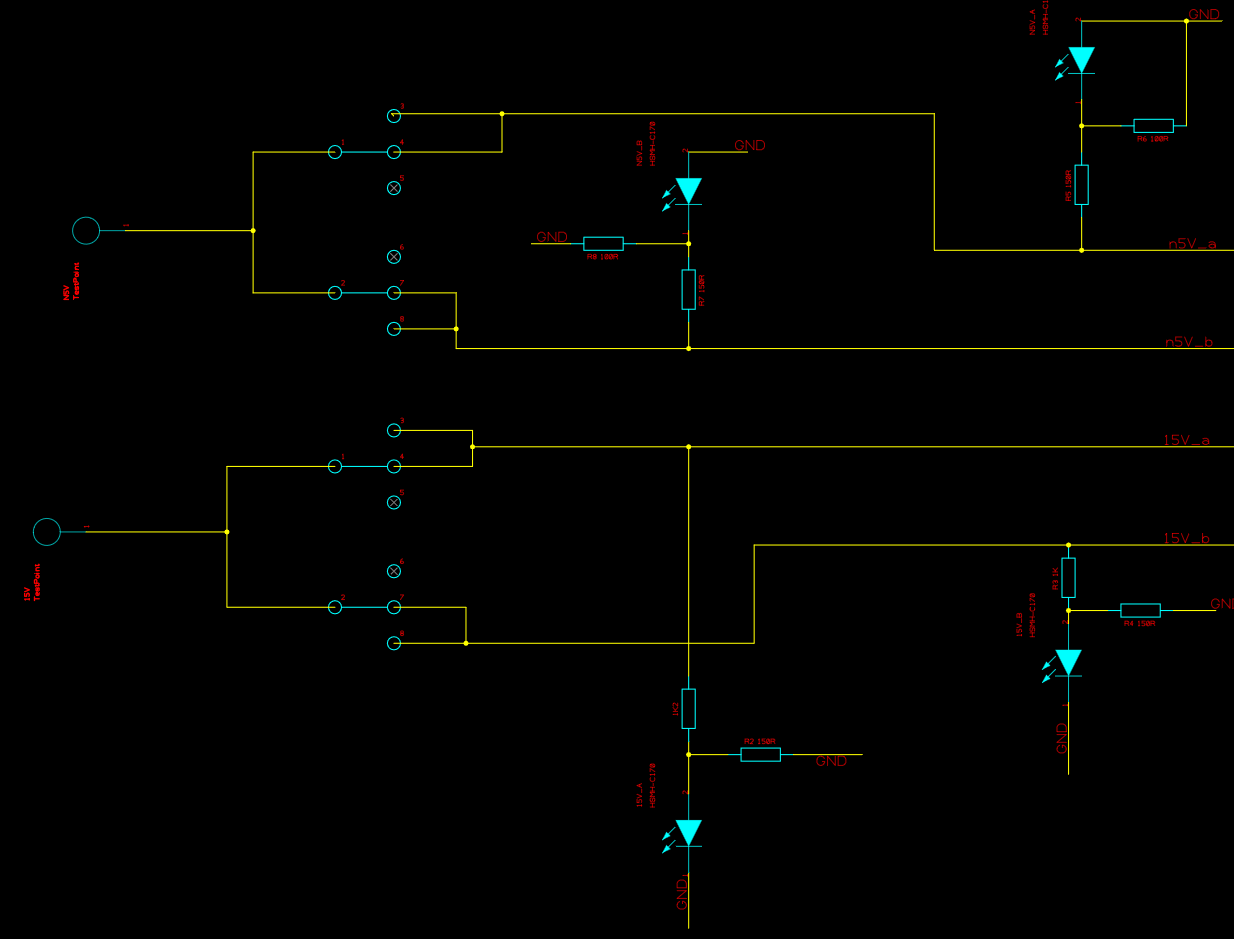
\includegraphics[width=\textwidth]{amp_top_power_indicators}
	\caption{Power indicator \& switching circuits for the -5V and +15V lines}
\end{figure}

\begin{figure}[!htb]
	\centering
	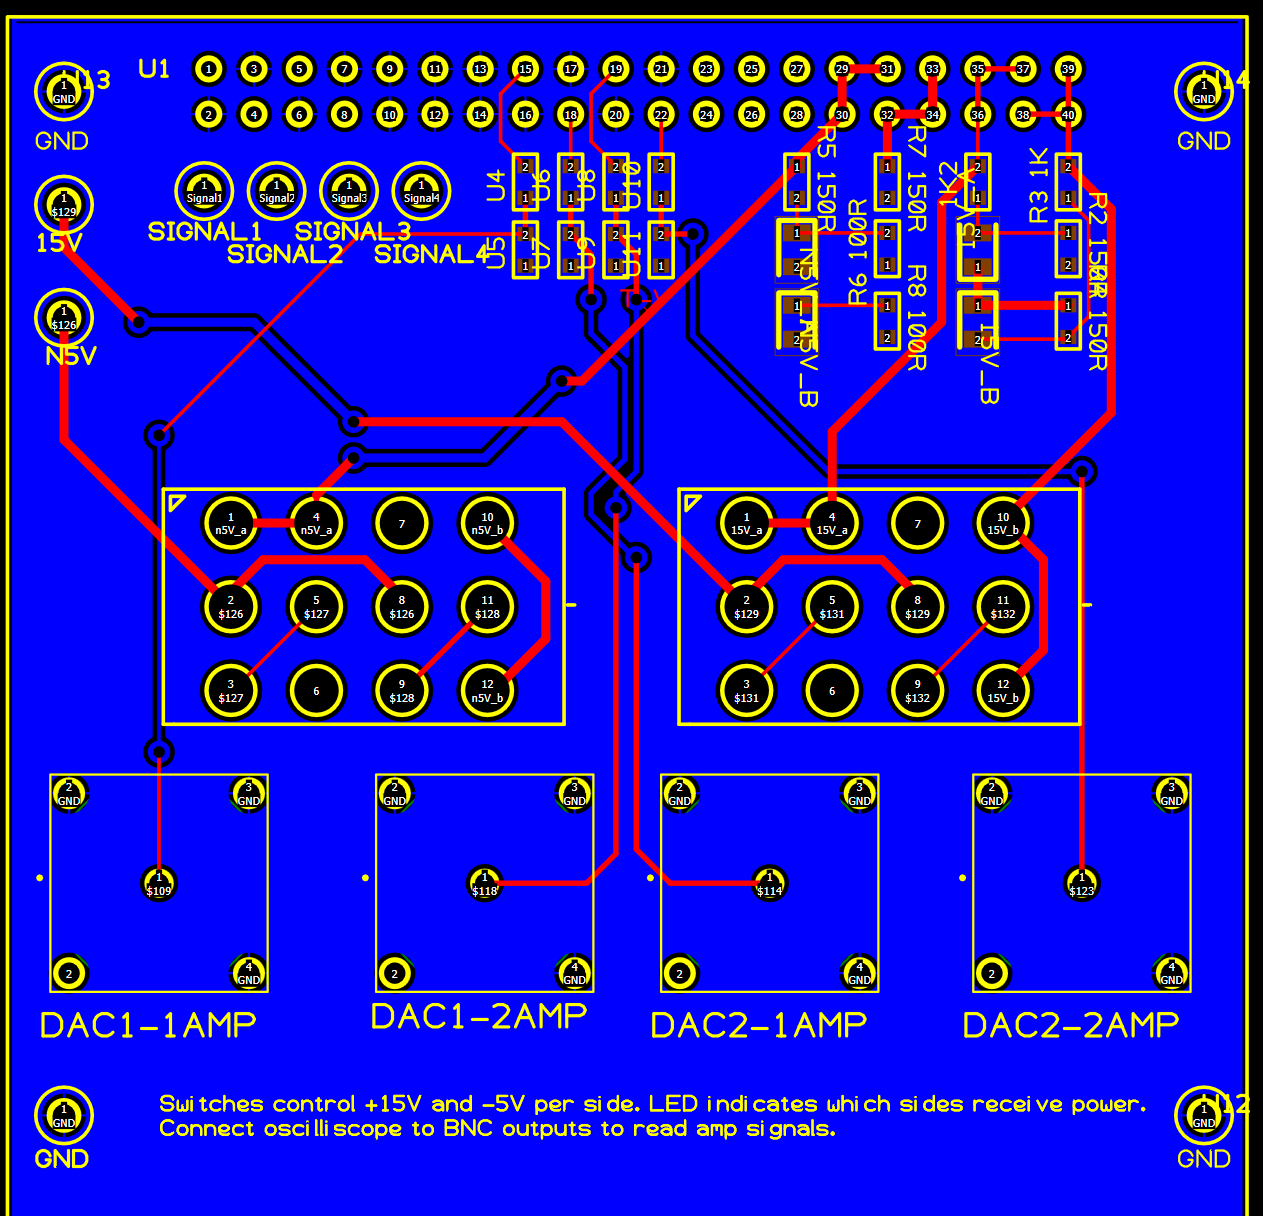
\includegraphics[width=0.7\textwidth]{amp_top_layout}
	\caption{Finished layout of Top testing board}
\end{figure}

\begin{figure}[!htb]
	\centering
	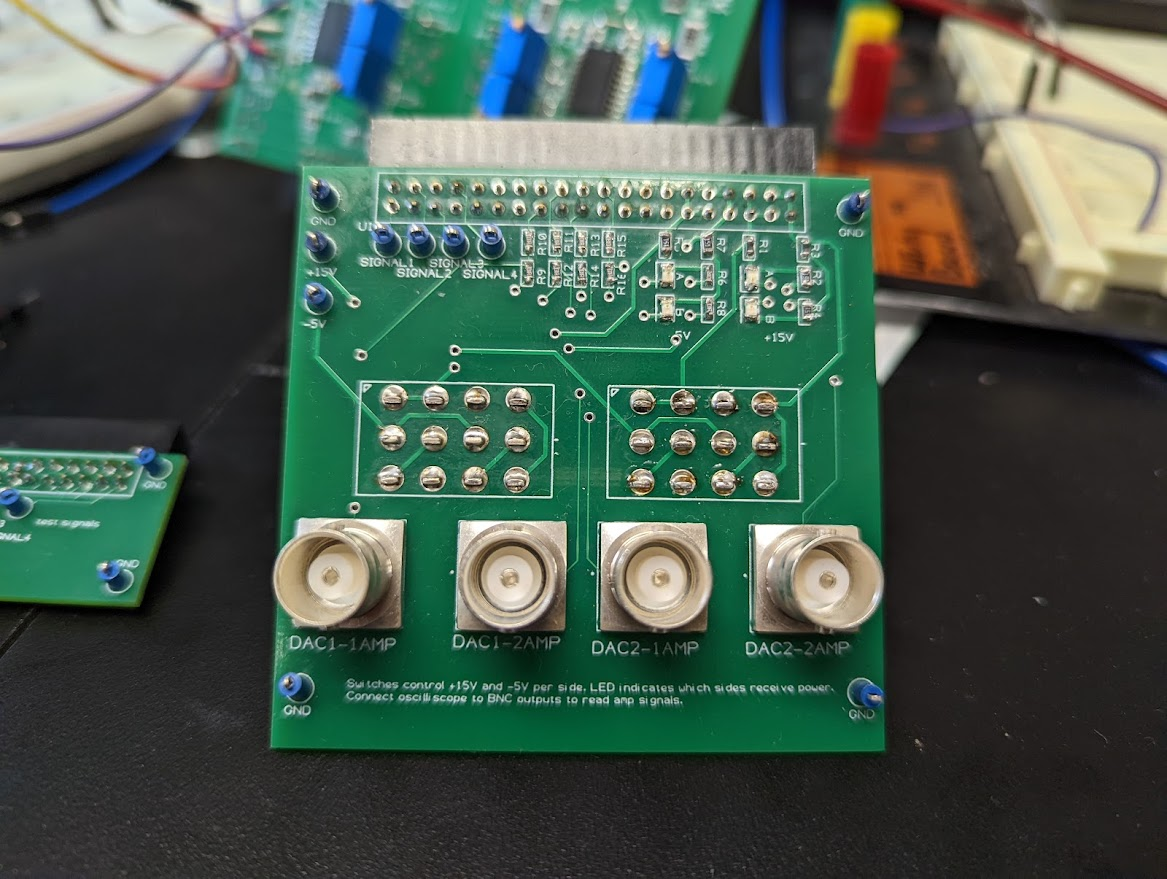
\includegraphics[width=\textwidth]{amp_top_board}
	\caption{Final fabricated Top test board}
\end{figure}

\begin{figure}[!htb]
	\centering
	\begin{subfigure}[b]{0.6\textwidth}
		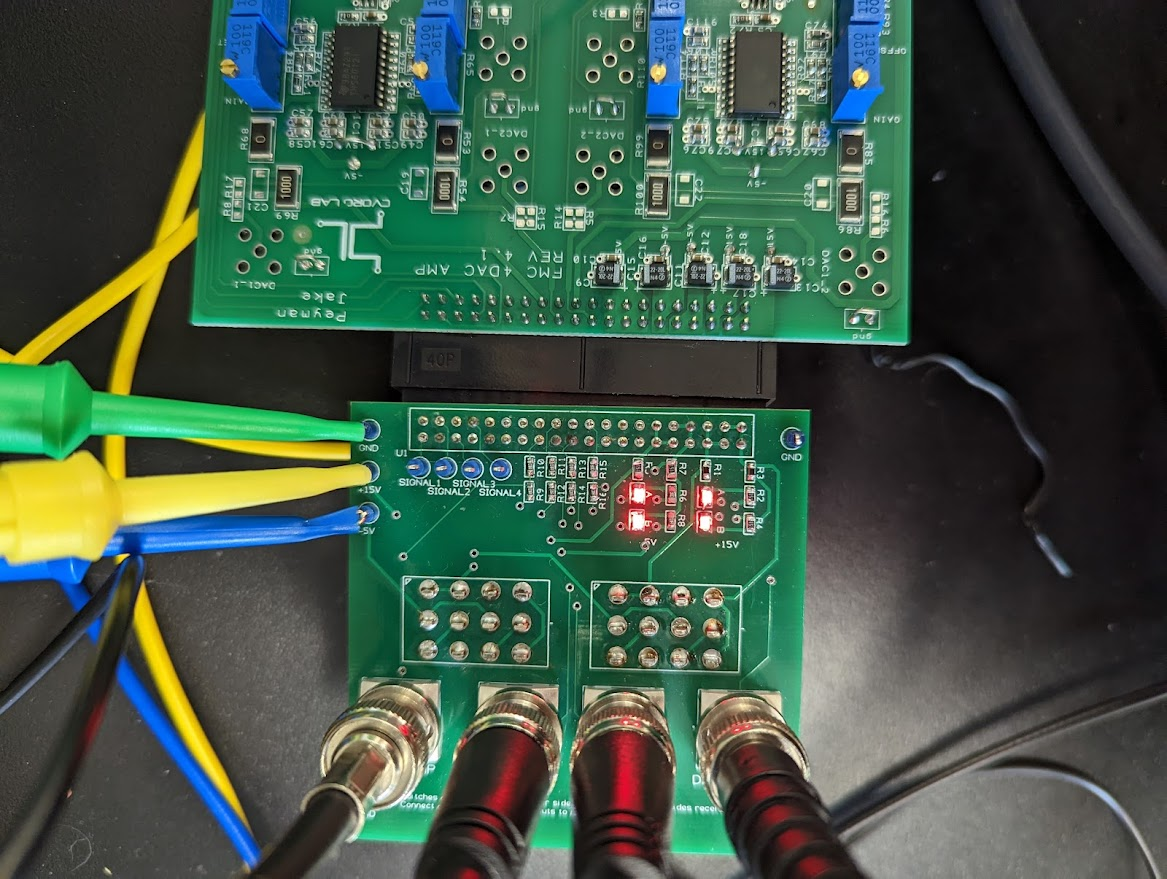
\includegraphics[width=\textwidth]{amp_power_leds}
		\caption{Power LED indicators}
		\centering
	\end{subfigure}
	\begin{subfigure}[b]{0.39\textwidth}
		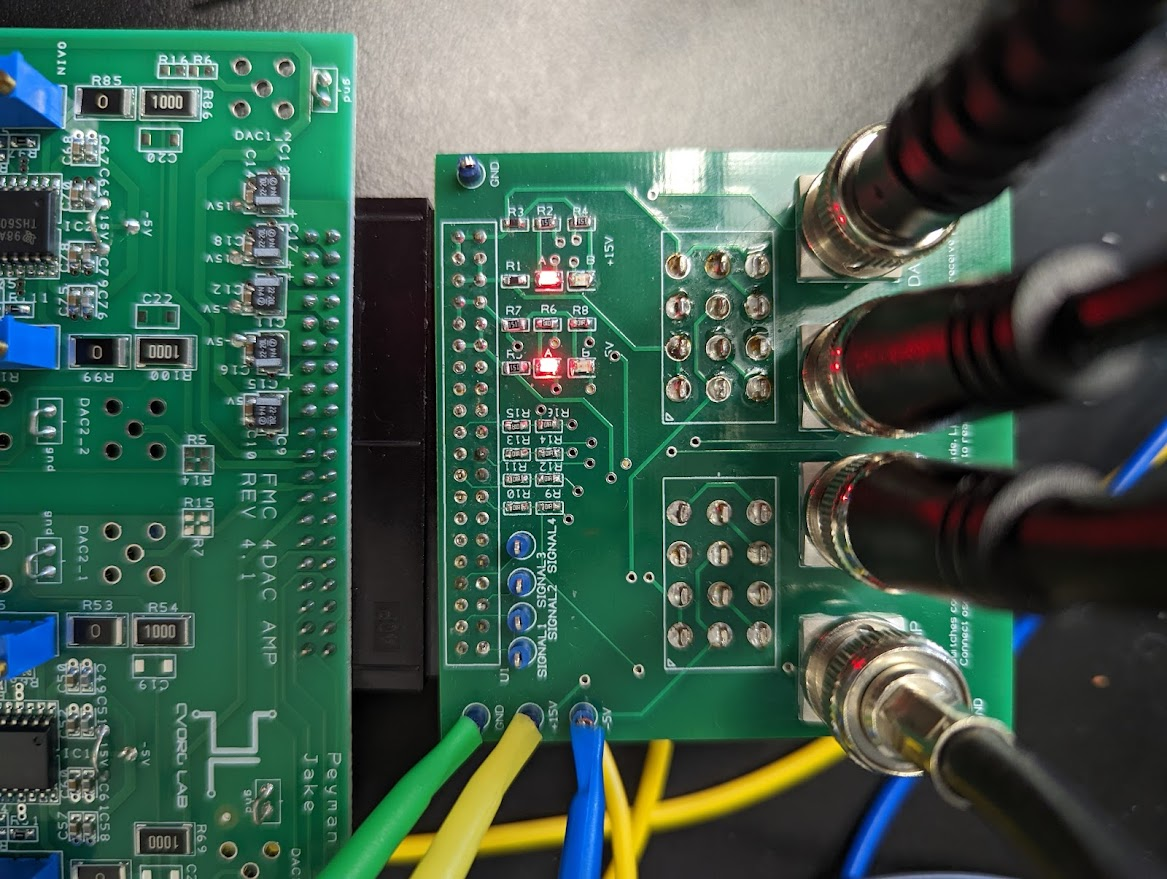
\includegraphics[width=\textwidth]{amp_top_a_powered}
		\caption{Only Amplifier A is on}
	\end{subfigure}
\end{figure}

\begin{figure}[!htb]
	\centering
	\begin{subfigure}[b]{0.49\textwidth}
		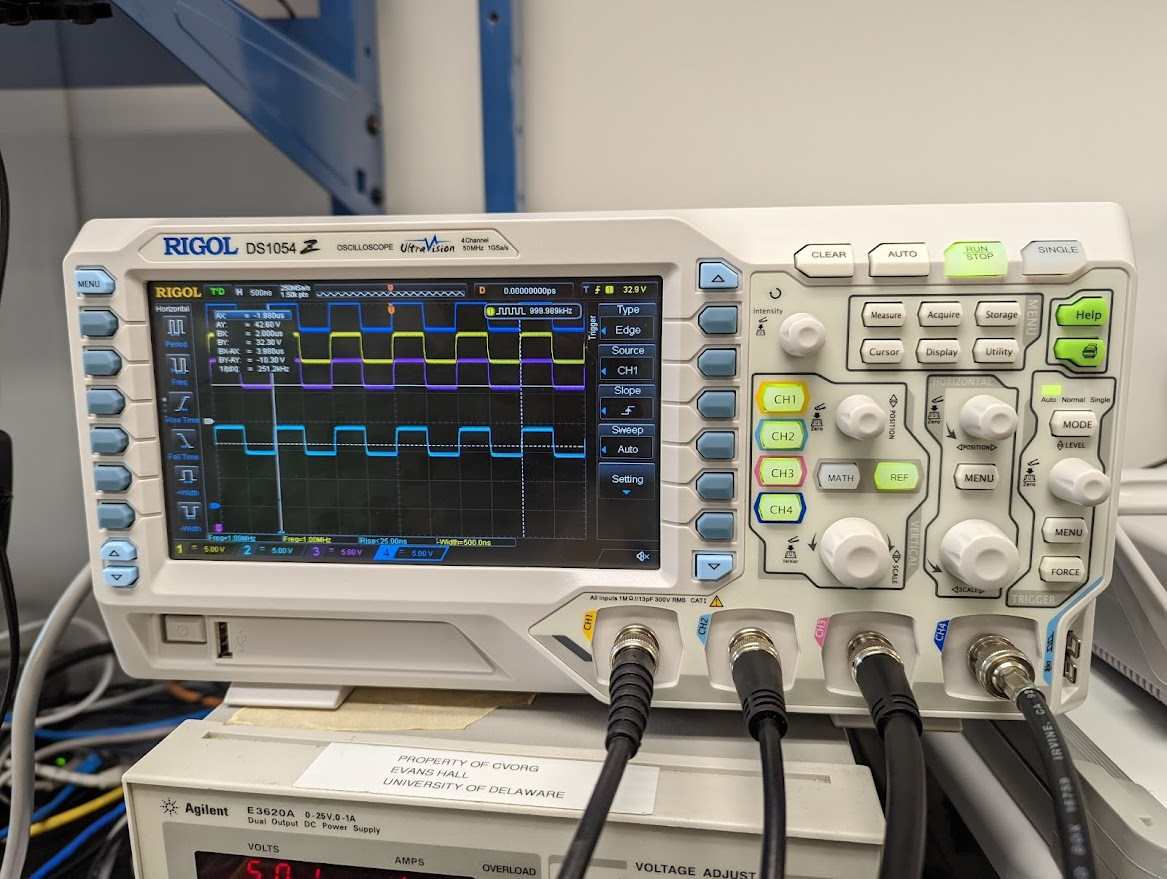
\includegraphics[width=\textwidth]{amp_scope_pre_programmed}
		\caption{Before programming, scope channels are not aligned}
	\end{subfigure}
	\begin{subfigure}[b]{0.49\textwidth}
		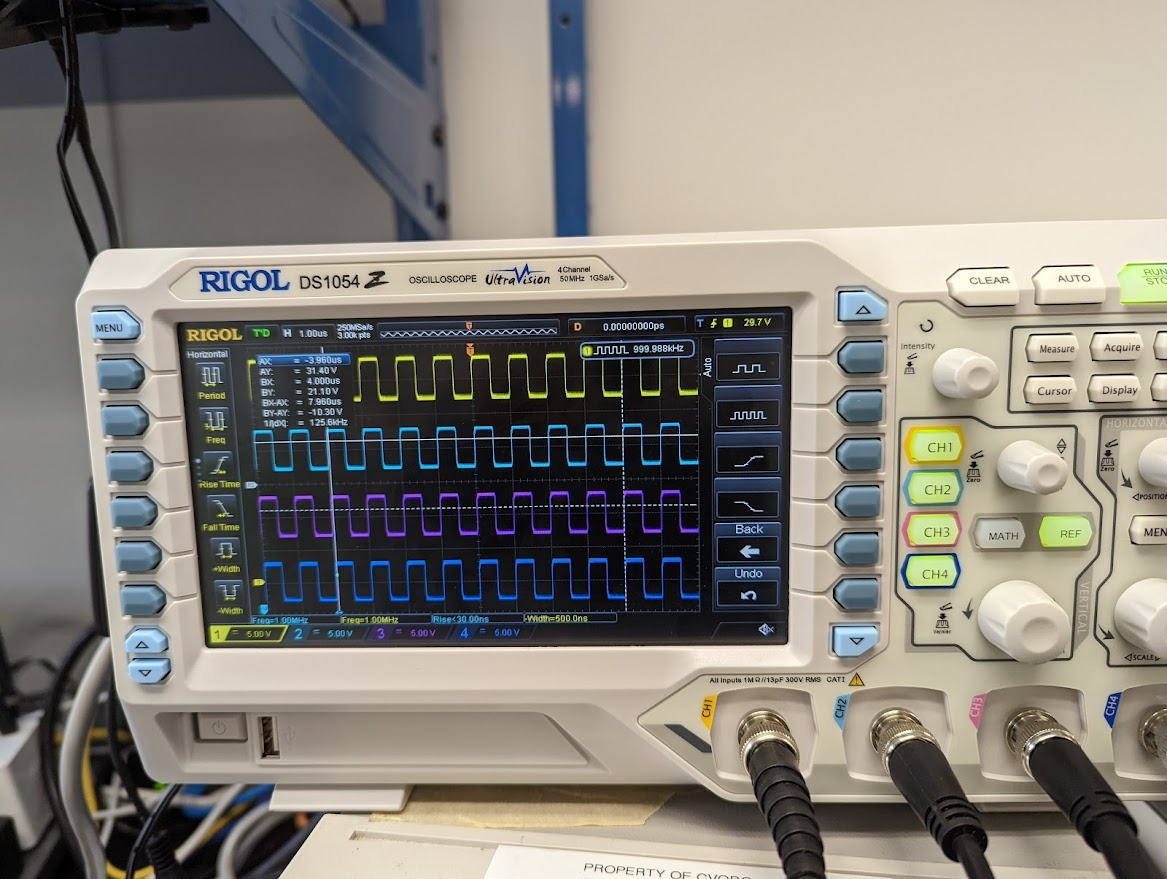
\includegraphics[width=\textwidth]{amp_scope_full_output.jpg}
		\caption{After programming, all signals are visible and ready for capture}
	\end{subfigure}
\end{figure}

\begin{figure}[!htb]
	\centering
	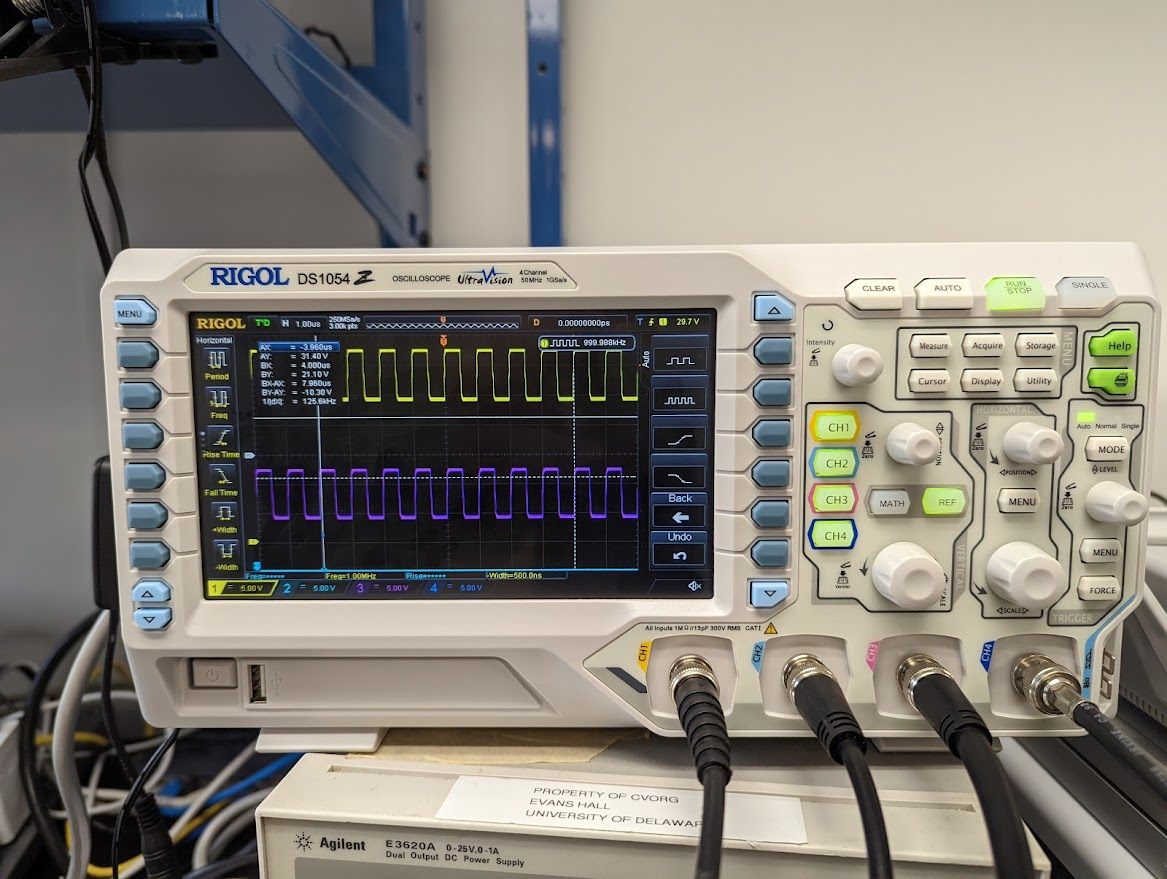
\includegraphics[width=\textwidth]{amp_scope_a_output}
	\caption{Scope output when only Side A is powered}
	\centering
\end{figure}


\section{Results}
\FloatBarrier
In order to reflect DACIN values I created arrays of amplitude values to be used by the AWG. By sweeping across the desired input range we could quickly gather data on the amplifiers without having to manually adjust inputs. The system operates with discrete sets of analog outputs and as such the measurements would be easy to gather within a predetermined window of time. The oscilloscope scale was fully programmable and allowed us to increase or decrease the number of samples on the screen. Boundaries were set according to the table values and arrays were created to record inputs and outputs. To sweep across a boundary, I created a function that stepped 100 times through the given voltage range.
\FloatBarrier
\begin{lstlisting}
	# DACIN = 9000
	dacin_9000 = [1.41, 1.53]
	x1 = []
	y1_1, y2_1, y3_1, y4_1 = []
	# DACIN = 13106
	dacin_13106 = [2.07, 2.18]
	x2 = []
	y1_2, y2_2, y3_2, y4_2 = []
	# DACIN = 19660
	dacin_19660 = [3.04, 3.16]
	x3 = []
	y1_3, y2_3, y3_3, y4_3 = []
	# DACIN = 26214
	dacin_26214 = [4.02, 4.16]
	x4 = []
	y1_4, y2_4, y3_4, y4_4 = []
	# DACIN = 32767
	dacin_32767 = [5, 5.2]
	x5 = []
	y1_5, y2_5, y3_5, y4_5 = []
\end{lstlisting}

\begin{lstlisting}
	def dacin_sweep(dacin_bounds, x, y1, y2, y3, y4, awg, scope):
    # turn off AWG
    awg.set_on_off(1, 0)
    awg.set_on_off(2, 0)
    # set scope parameters & turn on displays
    scope.display_channel("CHAN1", True)
    scope.set_probe_ratio("CHAN1", 10)
    scope.set_channel_scale("CHAN1", 5, False)
    scope.set_channel_offset("CHAN1", -20.20)

    scope.display_channel("CHAN2", True)
    scope.set_probe_ratio("CHAN2", 10)
    scope.set_channel_scale("CHAN2", 5, False)
    scope.set_channel_offset("CHAN2", -36.40)

    scope.display_channel("CHAN3", True)
    scope.set_probe_ratio("CHAN3", 10)
    scope.set_channel_scale("CHAN3", 5, False)
    scope.set_channel_offset("CHAN3", -24.70)

    scope.display_channel("CHAN4", True)
    scope.set_probe_ratio("CHAN4", 10)
    scope.set_channel_scale("CHAN4", 5, False)
    scope.set_channel_offset("CHAN4", -15.0)
    step = (dacin_bounds(1) - dacin_bounds(0)) / 100

    for i in range(100):
        x[i] = dacin_bounds(0) + step
        awg.set_waveform(1, 1)
        awg.set_frequency(1, 1000000)
        awg.set_amplitude(1, x[i])
        awg.set_offset(1, 0)
        awg.set_phase(1, 0)
        awg.set_on_off(1, 1)
        chan1 = scope.get_waveform_samples("CHAN1", "NORMal")
        chan2 = scope.get_waveform_samples("CHAN2", "NORMal")
        chan3 = scope.get_waveform_samples("CHAN3", "NORMal")
        chan4 = scope.get_waveform_samples("CHAN4", "NORMal")
        y1[i] = max(chan1) - min(chan1)
        print(y1[i])
        y2[i] = max(chan2) - min(chan2)
        print(y2[i])
        y3[i] = max(chan3) - min(chan3)
        print(y3[i])
        y4[i] = max(chan4) - min(chan4)
        print(y4[i])
        step += step
\end{lstlisting}
\FloatBarrier
Using this simple script the equipment was automated to set parameters and measure, storing the data in arrays to be plotted with numpy later. \par
Initial data collection was only performed with five input points and five outputs. While rudimentary, this served as an effective foundation for understanding larger-scale measurements and intensive voltage sweeps. In general, good cards would respond linearly to increasing voltage input. Examples of results from different cards are shown below:
\begin{figure}[!htb]
	\centering
	\begin{subfigure}[b]{0.4\textwidth}
		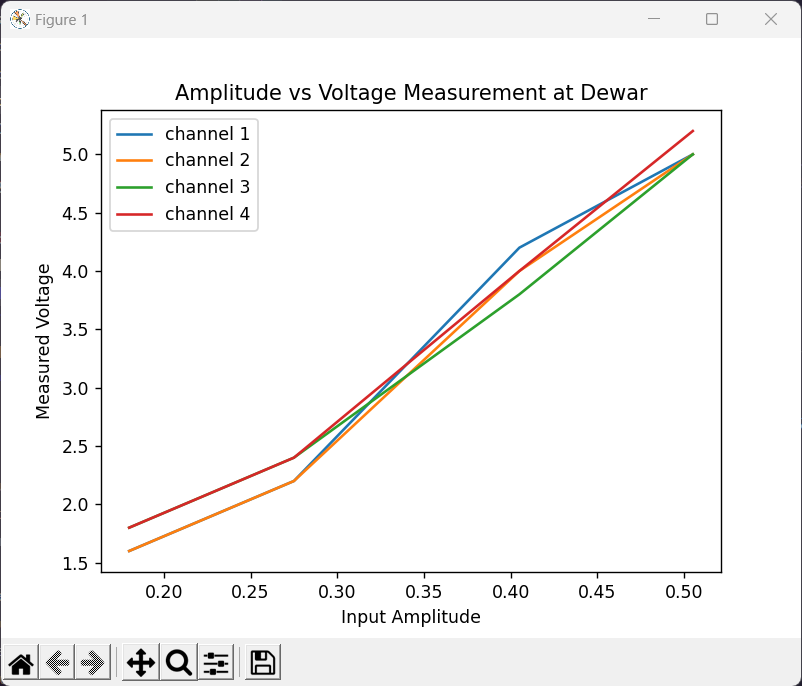
\includegraphics[width=\textwidth]{output_measurement}
		\caption{Best response}
	\end{subfigure}
	\begin{subfigure}[b]{0.4\textwidth}
		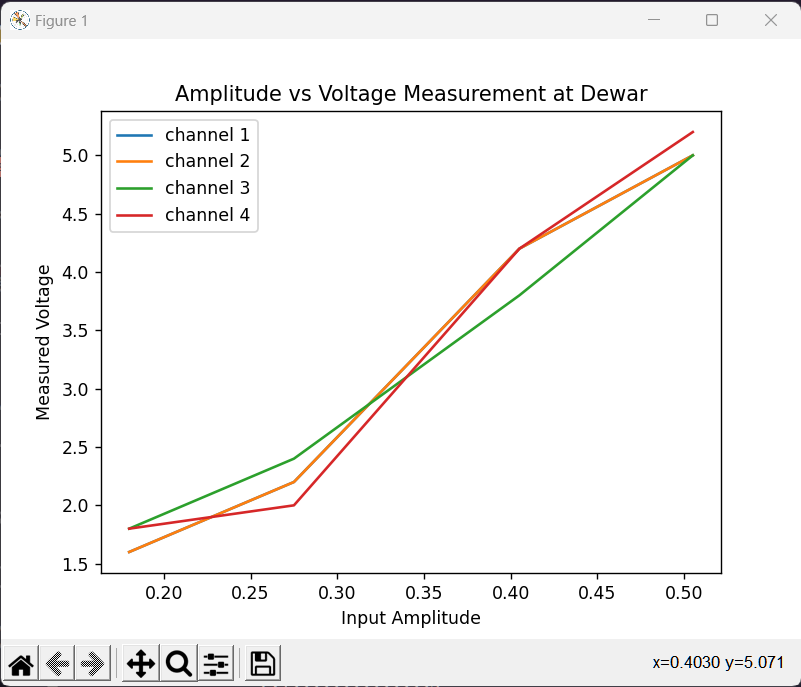
\includegraphics[width=\textwidth]{output_measurement2}
		\caption{Acceptable response}
		\label{graphb}
	\end{subfigure}
	\begin{subfigure}[b]{0.4\textwidth}
		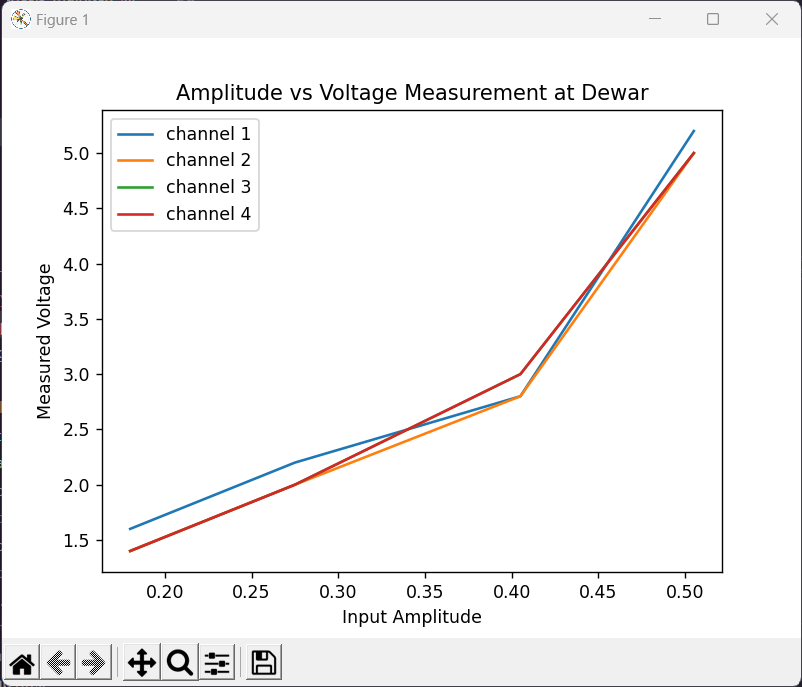
\includegraphics[width=\textwidth]{output_measurement3}
		\caption{Needs tuning}
	\end{subfigure}
	\caption{Results from three different amp sweeps}
\end{figure}
The graphs make diagnosing and parsing issues significantly easier. For example, \ref{graphb} shows a card that has somewhat irregular response across channels 2 and 4. This can easily be pointed to as an issue with the signals' driver, amplifier B. Identified in this way, the cards can quickly be touched up and re-tested.